% !TEX TS-program = xelatex
% !TEX encoding = UTF-8 Unicode 

% \documentclass[AutoFakeBold]{LZUThesis}
\documentclass[AutoFakeBold]{LZUThesis}
\usepackage{multirow}
\usepackage{threeparttable}
\usepackage{booktabs} % 导入三线表需要的宏包
\usepackage{longtable}% 导入跨页表格所需宏包


\CTEXsetup[name={第,部分}]{chapter}
\lstset{
language = MATLAB,
backgroundcolor=\color{white},   % choose the background color; you must add \usepackage{color} or \usepackage{xcolor}  
basicstyle=\footnotesize,        % the size of the fonts that are used for the code  
breakatwhitespace=false,         % sets if automatic breaks should only happen at whitespace  
breaklines=true,                 % sets automatic line breaking  
captionpos=bl,                    % sets the caption-position to bottom  
% commentstyle=\color{green},    % comment style  
% deletekeywords={...},            % if you want to delete keywords from the given language  
% escapeinside={\%*}{*)},          % if you want to add LaTeX within your code  
extendedchars=true,              % lets you use non-ASCII characters; for 8-bits encodings only, does not work with UTF-8  
frame=shadowbox,                    % adds a frame around the code  
keepspaces=true,                 % keeps spaces in text, useful for keeping indentation of code (possibly needs columns=flexible)  
keywordstyle=\color{blue},       % keyword style  
% language=Python,                 % the language of the code  
morekeywords={*,...},            % if you want to add more keywords to the set  
numbers=left,                    % where to put the line-numbers; possible values are (none, left, right)  
numbersep=5pt,                   % how far the line-numbers are from the code  
numberstyle=\tiny\color{gray}, % the style that is used for the line-numbers  
rulecolor=\color{black},         % if not set, the frame-color may be changed on line-breaks within not-black text (e.g. comments (green here))  
showspaces=false,                % show spaces everywhere adding particular underscores; it overrides 'showstringspaces'  
showstringspaces=false,          % underline spaces within strings only  
showtabs=false,                  % show tabs within strings adding particular underscores  
stepnumber=1,                    % the step between two line-numbers. If it's 1, each line will be numbered  
stringstyle=\color{orange},     % string literal style  
tabsize=2,                       % sets default tabsize to 2 spaces  
% title=signalAnalysis.m           % show the filename of files included with \lstinputlisting; also try caption instead of title  
}  

\begin{document}
%=====%
%
%封皮页填写内容
%
%=====%

% 标题样式 使用 \title{{}}; 使用时必须保证至少两个外侧括号
%  如: 短标题 \title{{第一行}},  
% 	      长标题 \title{{第一行}{第二行}}
%             超长标题\tiitle{{第一行}{...}{第N行}}

\title{{电子交通灯综合设计实验}}



% 标题样式 使用 \entitle{{}}; 使用时必须保证至少两个外侧括号
%  如: 短标题 \entitle{{First row}},  
% 	      长标题 \entitle{{First row}{ Second row}}
%             超长标题\entitle{{First row}{...}{ Next N row}}
% 注意:  英文标题多行时 需要在开头加个空格 防止摘要标题处英语单词粘连.

\author{\CJKfontspec{楷体}李文涛}
\major{电子信息基地班}
\college{320200928101}
\grade{2020级}



\maketitle
\frontmatter

%中文摘要
\ZhAbstract{
    本文主要介绍了对电子交通灯的功能需求进行分析的过程,将其功能拆分,利用模块化设计的思想
    将功能一步步实现,完成时钟信号产生模块、倒计时模块、红绿灯显示模块、倒计时数字化显示模块,
    然后将各功能模块组合在一起实验完整的电子交通灯系统。
    通过完整地进行对电子信号灯的设计,了解了电子设计的基本过程,具备初步独立设计电子系统的能力,
    认识到模块化设计和提前整体设计布局的重要性。
}
{电子交通灯,模块化设计,整体设计布局}


%英文摘要
\EnAbstract{This paper mainly introduces the process of analyzing the functional requirements of the electronic traffic light, splitting its functions and using the idea of modular design
The functions will be realized step by step, complete the clock signal generation module, countdown module, traffic light display module, countdown digital display module,
Then the functional modules are combined together to experiment the complete electronic traffic light system.
Through the complete design of the electronic signal lamp, I understand the basic process of electronic design, and have the ability to design the electronic system independently.
Recognize the importance of modular design and overall layout in advance.
    \fontspec{Times New Roman}}
{Electronic traffic lights, modular design, overall design layout}

%生成目录
% \tableofcontents
% \addcontentsline{toc}{chapter}{目录}
% \thispagestyle{empty}


%文章主体
\mainmatter

\chapter{明确设计目标}

\section{基本功能要求}

\subsection{具备四路交通信号}

即支持十字路口交通管理能力,具备四路交通信号。在设计的电路里,要将整个路口四个信号灯各自的状态整合,转化为“十字路口”
交通系统的整体状态,在这一部分,要认识到十字路口的四路信号其中两两对应,实际上也就是两路信号的整合。


\subsection{发光二极管作为信号灯}

在使用放光二极管作为信号灯时,要考虑到芯片的输出电流和电压能否驱动二极管发光的问题,
考虑到发光二极管所需的工作电流电压大于芯片输出电流电压,
我们要进行电路上的设计来解决驱动问题。

\subsection{显示转换倒计时}

要求能够显示红绿灯转换倒计时,根据生活中实际情况和当地红绿灯的显示状况,可以认为,
四路倒计时的时间是相同的,状态是红灯的那路在倒计时结束时直接变为绿灯,而状态是绿灯的
那路在倒计时剩余三秒时变为黄灯,归零时变为红灯。

\section{其他设计要求}
\subsection{考虑各参数的合理性}

在设置红黄绿灯的停留时间时应考虑车辆通过路口需要的时间;设置脉冲时,要注意其周期和占空比,
为了达到预期值需要测试更改信号发生模块各元器件的参数。

\subsection{仿真电路布局的合理性}

由于仿真电路往往是印制PCB电路或其他成品电路的设计参考,在芯片位置的布置和布线
上要具有条理,尽量使连线不交错,各模块布置的位置便于关联。
\chapter{预设计分析}

\section{总体模块布局}

\begin{figure}[htbp]
    \centering
    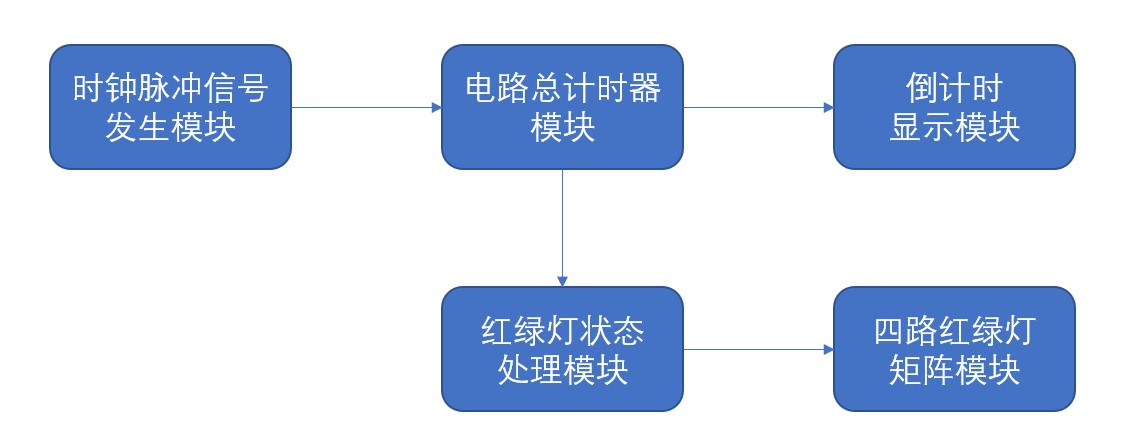
\includegraphics[keepaspectratio,width=380pt]{mokuai.jpg}
    \caption{总体布局模块图}
\end{figure}

\section{具体模块介绍}
\subsection{时钟脉冲信号发生模块}
根据所学知识,目标以555定时器制作周期为1s的矩形脉冲信号。

\subsection{电路总计时器模块}
控制整个系统的运行节奏,同时又是红绿灯状态变换信号的发出端,简单来说是在指定的时间将改变
信号灯状态的脉冲发送给红绿灯状态处理模块,并能够在设定的时间里进行循环运行。

\subsection{倒计时显示模块}
读取电路总计时器模块的时间信息,并通过七段译码管显示出来。

\subsection{红绿灯状态处理模块}
接收电路总计时器模块的脉冲信号改变红绿灯的的状态,
并且在这些状态中进行循环,
也就是我们可以设置一个计数器来表示其状态,并在接收到脉冲
时进行计数以进行状态的改变。
然后按照真值表使用逻辑电路去控制红绿灯的亮暗。

\subsection{四路红绿灯矩阵模块}
作为结果与红绿灯状态处理模块相接,直接显示十字路口的红绿灯状态。

\section{模块补充说明}
考虑到红绿灯的适用性,应该将两个走向的绿灯时间设置为用户可以调整的设计。
故在电路总计时器模块必须将信号的输入转为可控,从而导致我们需要对总计时器的预置时间
根据红绿灯所处状态改变。即在该模块要加入预设时间数据选择结构。

\chapter{电路拟真初步设计}

\section{时钟脉冲信号发生模块}
经查阅资料,了解555定时器生成脉冲的原理及参数的设置。
\begin{figure}[htbp]
    \centering
    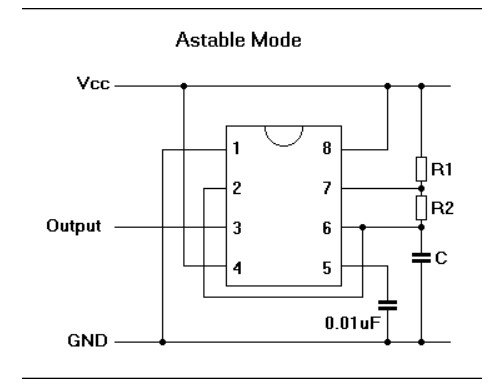
\includegraphics[keepaspectratio,width=310pt]{555.jpg}
    \caption{555定时器产生周期方波的电路示意图}
\end{figure}

其中,该电路的参数设置由以下公式决定:

\begin{equation}
    T_h=0.693\times (R_1+R_2) \times C
\end{equation}
\begin{equation}
    T_l=0.693\times R_2 \times C
\end{equation}
\begin{equation}
    f=\frac{1.44}{((R_1 + R_2 + R_2) \times C)}
\end{equation}
\begin{equation}
    DCP=(\frac{T_h}{T_h+T_l})\times 100
\end{equation}

以上$T_h$和$T_l$分别为一个周期中高电平和低电平的时间,$f$为输出信号的频率,
$DCP$为该信号的占空比。

通过计算,我们设置$R_1$为$400\Omega$, $R_2$为$7000\Omega $,
$C$为$0.1\mu F$。以此来产生我们所需的占空比近似于$50\%$,周期
为$1s$的矩形脉冲信号。

\begin{figure}[htbp]
    \centering
    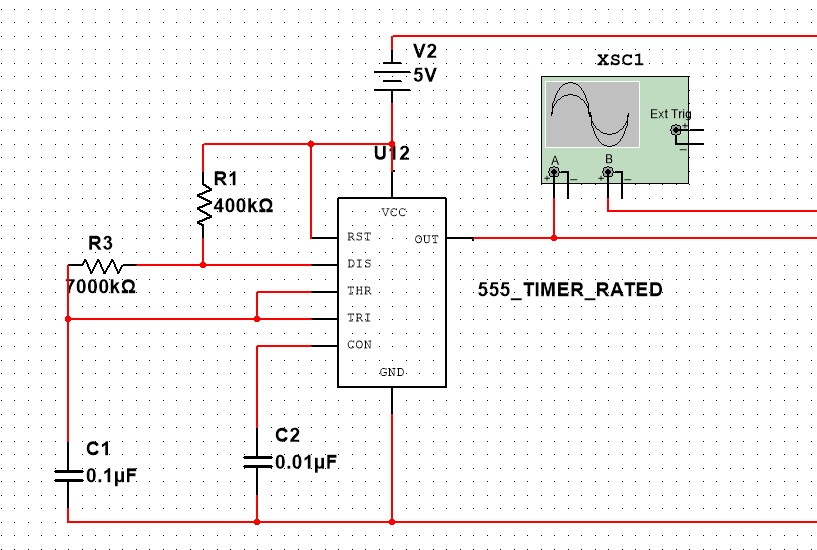
\includegraphics[keepaspectratio,width=280pt]{555m.jpg}
    \caption{555定时器周期方波电路仿真图}
\end{figure}
如下图所示,经示波器与标准方波信号对比,我们的矩形波产生电路在误差允许
的范围内能够达到预期要求。
\begin{figure}[htbp]
    \centering
    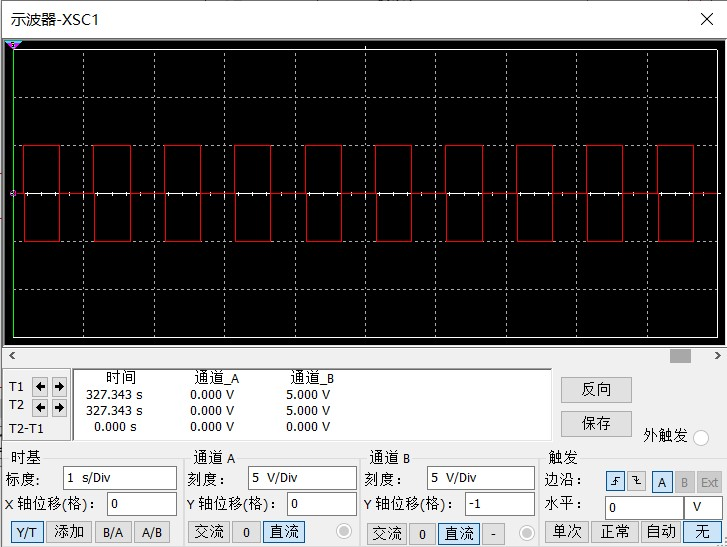
\includegraphics[keepaspectratio,width=280pt]{555p.jpg}
    \caption{555定时器周期方波对比图}
\end{figure}
\section{电路总计时器模块}
考虑到该模块需要和倒计时显示模块进行连接输出,故需要个十位分别输出,
根据数电课所学知识,利用74LS160芯片串联可以形成十进制的两位数字计数信号,
根据这一思路,我利用其特性将两片74LS160组合,并在该电路计数状态为“26”和“29”时通过
基本逻辑电路输出脉冲,同时在“29”时对系统进行置零。

\begin{figure}[htbp]
    \centering
    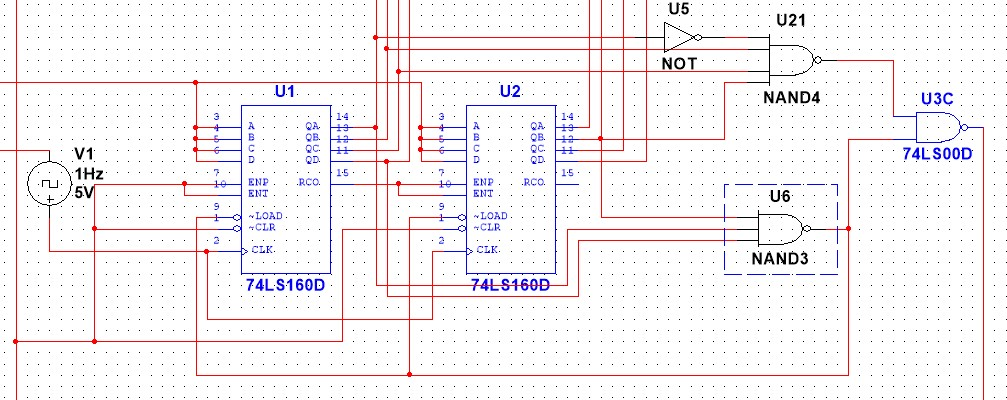
\includegraphics[keepaspectratio,width=320pt]{74160.jpg}
    \caption{74LS160芯片倒计时电路}
\end{figure}

同时考虑到倒计时输出,利用74LS181芯片的减法功能来进行倒计时的显示。

这里是将个位设置为9,十位设置为2,将其作为被减数,令$S_0$-$S_3$电平设置为
0110,$CN$和$M$设置为低电平,即算术减法运算,输出的个位和十位从各自的$F_0$-$F_3$
传输给译码管。

\begin{figure}[htbp]
    \centering
    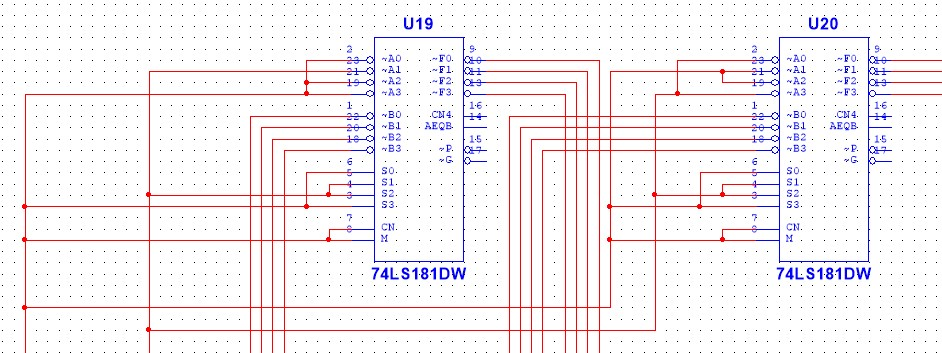
\includegraphics[keepaspectratio,width=320pt]{74181.jpg}
    \caption{74LS181芯片倒计时电路}
\end{figure}

\section{倒计时显示模块}
根据设计的布局,四个路口的倒计时显示应该是相同的,只需要将电路总计时器模块的倒计时信号
引出并连接至七段数字译码管即可。

\begin{figure}[htbp]
    \centering
    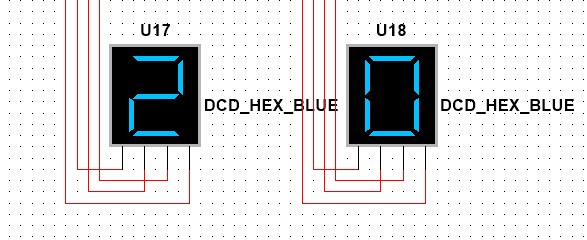
\includegraphics[keepaspectratio,width=250pt]{qiduan1.jpg}
    \caption{七段译码管连接示意图}
\end{figure}

\section{红绿灯状态处理模块}
这部分模块代表着整个电路的状态,我们首先对十字路口红绿灯状态进行分析:

首先红绿分为两个走向,每一个走向上的一对信号灯显示应该是相同的,这样一来,
我们十字路口信号灯的状态输出就应该是6盏红绿灯的亮暗。

这里为了方便说明,假设十字路口的走向都是正对东西南北的。

状态一:南北走向为红灯,东西走向为绿灯,南北走向禁止通行,东西走向允许通行。

状态二:南北走向为红灯,东西走向为黄灯,南北走向禁止通行,东西走向预告禁止通行。

状态三:南北走向为绿灯,东西走向为红灯,南北走向允许通行,东西走向禁止通行。

状态四:南北走向为黄灯,东西走向为红灯,南北走向预告禁止通行,东西走向禁止通行。

以上方状态为根据做出电路的真值表。
\begin{table}[!ht] % [!ht]表格在文本中放置的位置参数(努力放在当前位置,实在放不下,将放在下一页的顶部)
    \centering % 表格整体居中
    \caption{红绿灯状态真值表}
    \begin{tabular}{|c|c|c|c|c|c|c|c|} \hline % 其中,|c|表示文本居中,文本两边有竖直表线。
    电路状态(二进制$Q_2Q_1$) & 红灯$X_1$ & 黄灯$Y_1$ & 绿灯$Z_1$ & 红灯$X_2$ & 黄灯$Y_2$ & 绿灯$Z_2$   \\ \hline
    11 & 1 & 0 & 0 & 0 & 0 & 1  \\ \hline
    00 & 1 & 0 & 0 & 0 & 1 & 0 \\ \hline
    01 & 0 & 0 & 1 & 1 & 0 & 0 \\ \hline
    10 & 0 & 1 & 0 & 1 & 0 & 0 \\ \hline
    \end{tabular}
    \end{table}

根据上表,得到电路状态与红绿灯对应的逻辑关系:
\begin{align}
    X_1=Q_2Q_1+\overline{Q_2}\overline{Q_1}  \quad 
    Y_1=Q_2\overline{Q_1} \quad 
    Z_1=\overline{Q_2}Q_1\nonumber \\
    X_1=\overline{Q_2}Q_1+Q_2\overline{Q_1}  \quad 
    Y_1=\overline{Q_2}\overline{Q_1} \quad 
    Z_1=Q_2Q_1\nonumber
\end{align}

(PS:上式中的非均为$Q_2Q_1$各自的非)

通过简单逻辑运算电路连接得到输出,如下所示。

\begin{figure}[htbp]
    \centering
    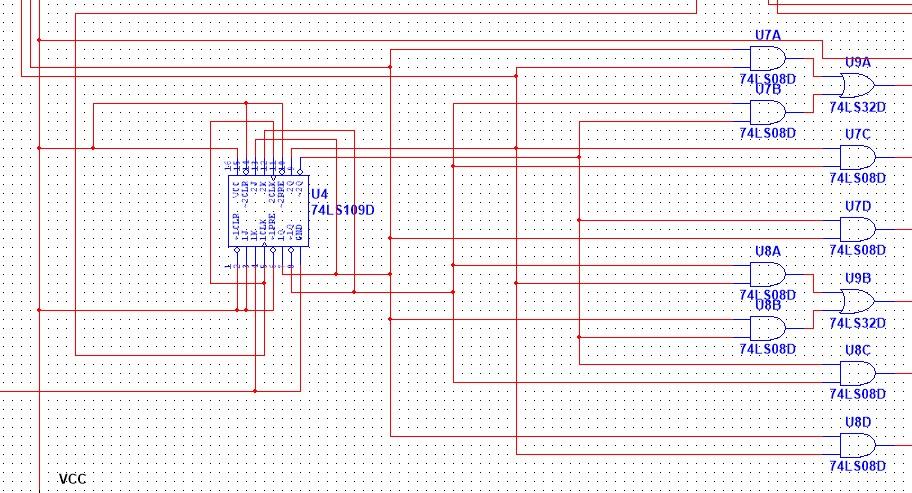
\includegraphics[keepaspectratio,width=320pt]{74109.jpg}
    \caption{红绿灯状态模块连接示意图}
\end{figure}


\section{四路红绿灯矩阵模块}
作为结果与红绿灯状态处理模块相接,直接显示十字路口的红绿灯状态。

\begin{figure}[htbp]
    \centering
    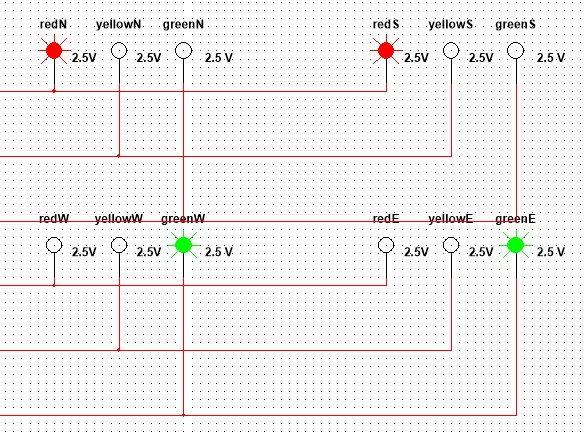
\includegraphics[keepaspectratio,width=250pt]{rgb1.jpg}
    \caption{红绿灯显示矩阵连接示意图}
\end{figure}
以上为红绿灯模拟连接示意图,以此保持电路图的合理性和可读性,也能够直观
显示红绿灯系统是由两对信号灯组成的。
\chapter{电路拟真改进设计}
\section{系统泛用性和用户的可操作性}
我们都知道,在实际生活中,根据实际交通状况,两个走向的允许通行的
时间要因需改变,所以我们要对原本的电路进行改进。

为了实现通行的时间即计数器的循环时间改变,我们可以对74LS181和74LS160的置数端进行改进,
引入数据选择器来识别红绿灯的状态以控制不同的置数,根据这个思路我在对电路改进时发现了一个问题。
原本为了避开74LS181在进行减法时出现负数的情况,我将倒计时个位都设置为了9,
但如果改为用户自行调整便无法避免这个问题,
同时又因为74LS181和74LS160的组合倒计时不仅会出现置数上的匹配问题,还会
使电路变得复杂。
怎么解决这个问题并实现用户的可调整的倒计时呢?
这时我发现了74LS190芯片能够解决这一问题。

74LS190芯片作为一款和74LS160有相似之处的芯片,它并不在我之前了解的芯片知识内,
经查阅资料,74LS190芯片除了能够做到74LS160的置数操作,还可以根据功能端的信号
来进行倒计时操作。在满足了我们的需求的情况下,还简化了电路。

\begin{figure}[htbp]
    \centering
    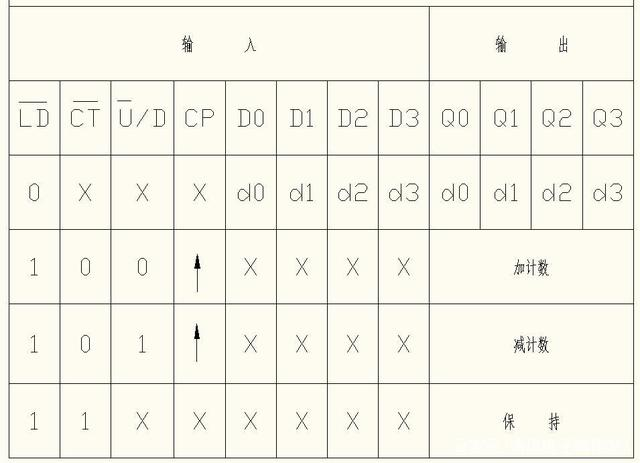
\includegraphics[keepaspectratio,width=280pt]{74190.jpeg}
    \caption{74LS190功能表}
\end{figure}

根据74LS190芯片的功能表,我们进行电路的设计,首先将两个74LS190进行串联构成
100进制的递减计数器,将$\overline{U}/D$端接高电平以达到减计数的效果,
通过将控制个位的74LS190芯片的$\overline{RCO}$端口接至
控制十位的芯片的$\overline{CT}$端控制十位的变化。

\begin{figure}[htbp]
    \centering
    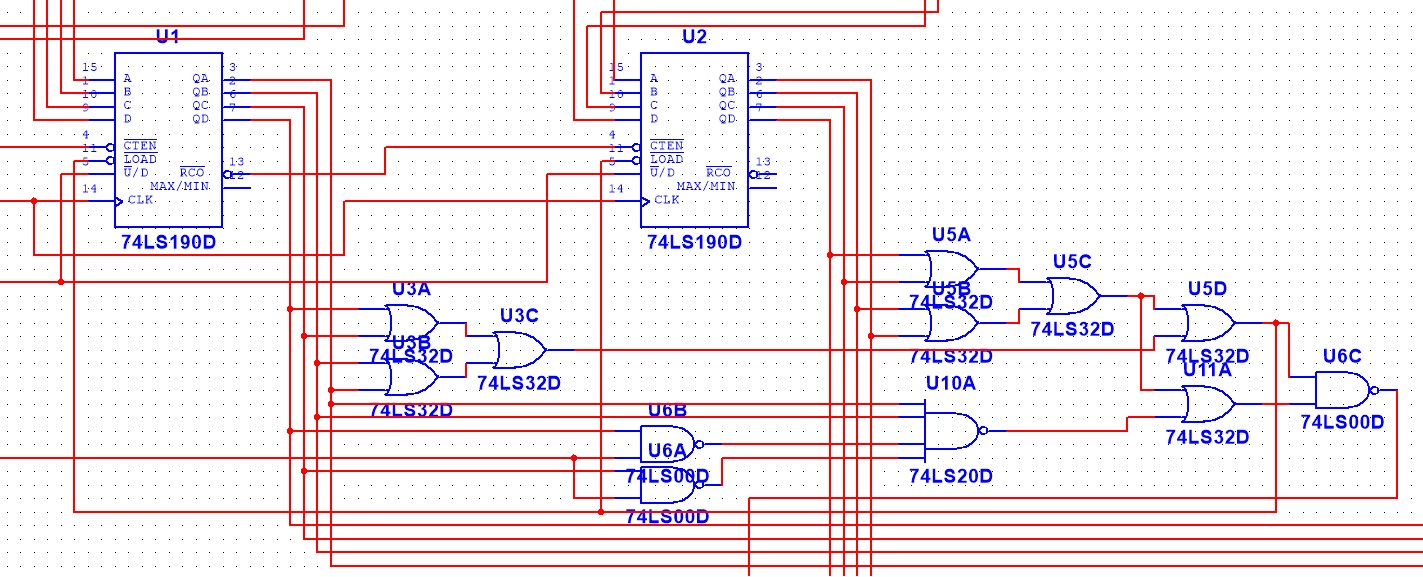
\includegraphics[keepaspectratio,width=330pt]{74190s.jpg}
    \caption{计时器模块部分电路图}
\end{figure}

同时为了能够给红绿灯状态处理模块提供脉冲,我们对该计数器的输出端进行选择,找出合适的
状态并在该状态下能够对状态处理模块输出脉冲信号,这里我们利用与非门和或门进行逻辑运算,
这里我选择了电路的“00”和“03”状态作为产生脉冲信号的状态。选择“00”状态时我将8条数据
输出全部用或门连接起来,这样就得到一个仅有在电路状态为“00”时才会输出低电平的信号;
选择“03”时,个位我采用与非门结构,在个位电路状态仅在“1100”时才会输出低电平,与十位的
四位信号或关系后的信号再进行逻辑或,这样就得到了电路状态在“03”时才会输出低电平的信号。
接着将这两个信号用与非门连接,就达成了电路在这两个状态下输出高电平脉冲的效果。

接下来我们考虑置数的问题,将识别“00”的信号接入$\overline{LOAD}$,这样就能够做到在倒计时归零时重新置入
用户预设的通行时间。

而要做到两个走向的通行时间不同,就必须要求电路能够在不同的红绿灯状态下改变置数端的数字,
这里我选择采用数据选择器来实现这一效果。

我采用的是4选1数据选择器,观察之前我们得到的红绿灯的状态真值表,在电路状态为“00”和“10”切换不同的置入时间,
同时考虑到计数器的启动,将“11”和“10”接入相同的数字,来达到初始化置入数字和电路状态循环的效果。

\begin{figure}[htbp]
    \centering
    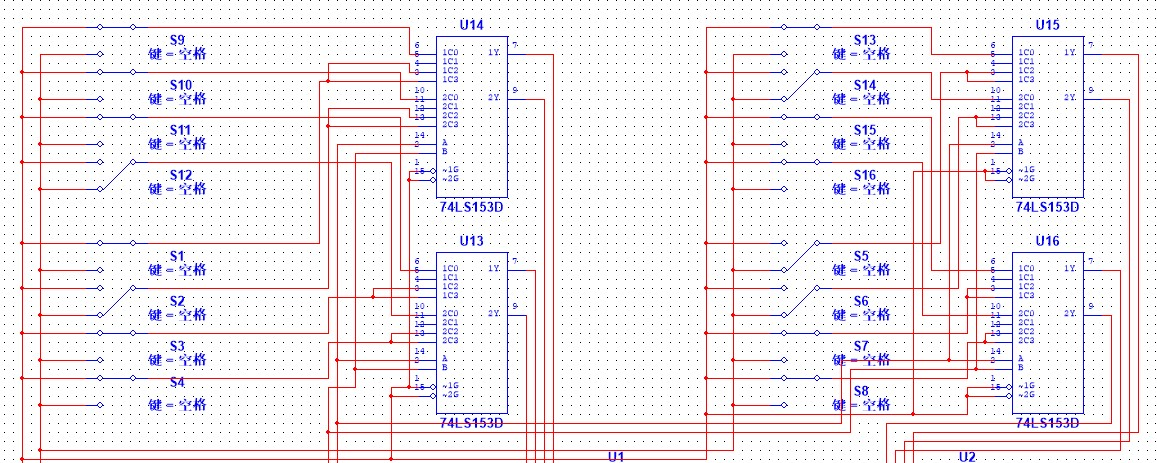
\includegraphics[keepaspectratio,width=450pt]{74153.jpg}
    \caption{计时器置数部分电路图}
\end{figure}
以上四部分从左上、左下、右上、右下的开关依次是控制南北走向倒计时的个位、东西走向
倒计时的个位、南北走向倒计时的十位、东西走向倒计时的十位。图中此时南北走向为28s,
东西走向为32s。(此处东西南北走向仅用于区分走向)
\section{电路实际驱动问题}
在进行数电学习时,学到了芯片输出的电压和电路是有限的,在我们实际驱动红黄绿发光二极管时,
会遇到电流或者电压不足而无法将二极管点亮的情况,这里我们采用引入上拉电阻的方法来解决。
具体电路如下所示。

\begin{figure}[htbp]
    \centering
    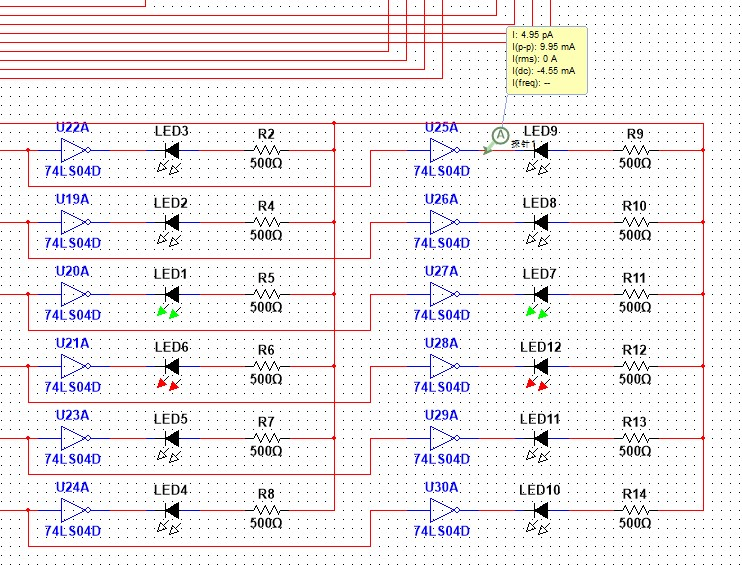
\includegraphics[keepaspectratio,width=400pt]{rgb2.jpg}
    \caption{红绿灯显示电路图}
\end{figure}

在输出后接反相器从总电源引来5v电压,经上拉电阻后与LED串联,这样就可以解决
实际电路中芯片输出电压电流无法驱动发光二极管的问题。

\chapter{实验设计总结及反思}
\section{小结}
至此,该电子交通灯的设计已基本完成,下方是目标设计电路。

\begin{figure}[htbp]
    \centering
    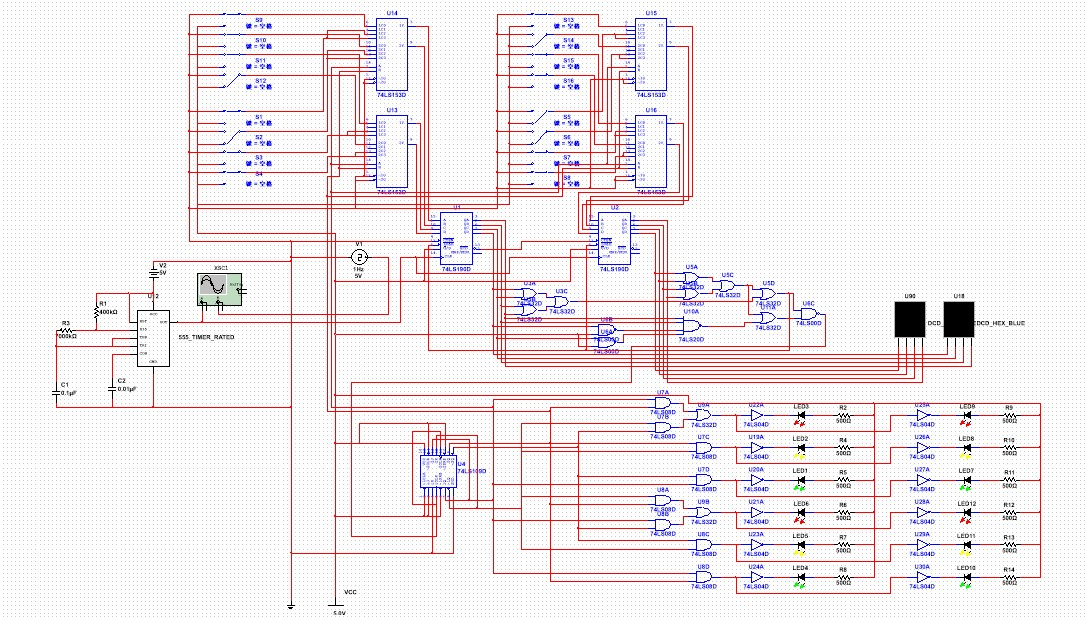
\includegraphics[keepaspectratio,width=450pt]{rgb3.jpg}
    \caption{电子交通灯电路图}
\end{figure}
在设计电路时,留意了布线的合理性,将各模块的供电,集合在一处,也方便真正作为产品
实现,在电路还滞留着标准脉冲信号和示波器,方便他人查阅,信号发生模块为了保持信号的
稳定,采用了独立的5V供电。
\section{对于倒计时显示的一些思考}
在开头设计分析时,我们对倒计时的显示做了目标预测,设想在规定的时间仅信号灯的颜色
改变,但并不改变绿灯转变为红灯之间的时间。这里就有一种分歧:

要不要把绿灯和黄灯的时间分开进行倒计时显示呢?
我们知道,在一路红灯而另一路绿灯时,红灯的时间是等于绿灯加黄灯的时间的。有些地区也确实
将绿灯和黄灯的倒计时分开,要不要对电路进行改进呢?

我认为如果将倒计时分开,除了要多加一组译码管外,如果不加其他倒计时系统的话,绿灯的显示时间
就是用绿灯转变为红灯的时间减去我设置的三秒黄灯,这时就需要一个算术运算来完成显示,可能会出现相减为
负的情况,而且这个减三秒的运算还需要通过对电路的状态进行判断,
来确定此时该译码管是显示的绿灯到红灯的时间还是红灯到绿灯的时间。

以此,由于最开始的设计目标的确定,在后面进行改进出现了问题,不易将绿灯和黄灯的倒计时分别
进行显示,但我们可以将倒计时的颜色进行改变。

这里,我选择数据分配器,通过对电路状态的识别,将倒计时信号送入不同颜色的译码管来达到目标。

\begin{figure}[htbp]
    \centering
    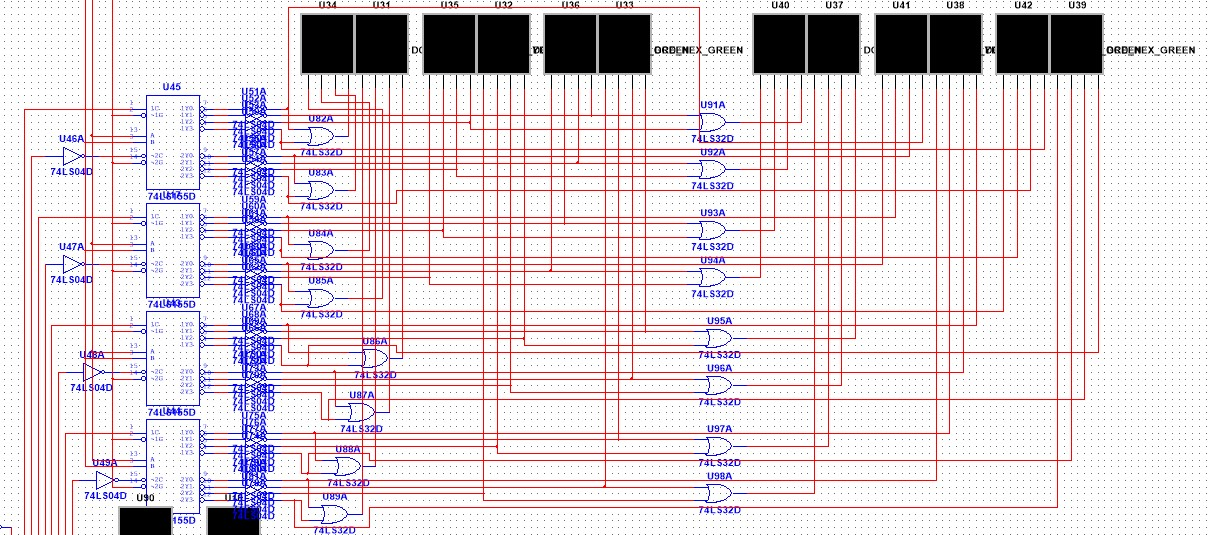
\includegraphics[keepaspectratio,width=450pt]{74155.jpg}
    \caption{交通灯倒计时显示电路图}
\end{figure}

简单介绍上面电路,就是通过74LS151芯片的数据分配选通不同的线路,利用简单的组合逻辑电路将信号分配给不同的译码管,
以达到倒计时颜色的变化。

但该电路的结构十分冗杂,严重影响整体的平衡性,会造成延迟和实物成本提高等问题,故作为备选方案提供。
\section{设计反思}
最终设计电路优点:电路简单易于理解,所用器材较少,布线较为清晰,用户可控倒计时时间,电路稳定性高;电路缺点:不能够显示
绿灯和黄灯各自的倒计时,初始状态可能会与实际状态有出入。

通过这次电子信号灯的设计,我基本掌握了器件电子设计的基本过程,
深刻意识到开始设计前做好对整体目标布局的重要性以及模块化分析的可操作性。
在之后的电子设计时,能够认真做好提前布局,了解更多的功能芯片,以做到更加合理并且
能够完成目标的电子设计。
\backmatter


% %=======%
% %引入参考文献文件
% %=======%
\bibdatabase{bib/POC}%bib文件名称 仅修改bib/ 后部分
\printbib
\nocite{*} %显示数据库中有的,但是正文没有引用的文献


% \Appendix

% 这里是附录页,可要可不要

% \Thanks.



\end{document}